\documentclass[letter, 12pt]{article}
\usepackage{latexsym}
\usepackage{amssymb,amsmath}
\usepackage[pdftex]{graphicx}
\usepackage{url}
\usepackage{mathtools}
\usepackage[square, numbers, comma,sort&compress]{natbib}
\usepackage{fancyhdr}
\usepackage{tikz}
\usepackage{upgreek}
\usepackage{multirow} 
\usepackage{setspace} 
\usepackage{datetime}
\usepackage[colorlinks,linkcolor=black,anchorcolor=blue,citecolor=blue]{hyperref}
\usepackage{bm}
\usepackage{threeparttable}
\usepackage{booktabs}
\usepackage[margin=2cm]{geometry}
\usepackage{xcolor}
\usepackage{subcaption}
\usepackage{colortbl}
\usepackage{multirow}
\definecolor{mygray}{gray}{.9}
% \usepackage{pdfpages}
\usepackage{algorithm}
\usepackage{algorithmic}
\usepackage[font=small,labelfont=bf]{caption}
\usepackage{setspace}

% 添加行距
\setstretch{1.5}

% keywords command
\providecommand{\keywords}[1]
{
  \small	
  \textbf{\textit{Keywords---}} #1
}

\include{format}

\pagenumbering{gobble}

\begin{document}


\begin{figure}
	\centering
	%	\setlength\fboxsep{0.5pt}
	%	 \fbox{
\includegraphics[width=4.5in]{./figure/Title.jpg}}
	
\includegraphics[width=4.5in]{./figs/Title.jpg}
\end{figure}
\title{\bf Proposal of DNN-based Wildfire Detection with UAV}
\author{\\ \normalsize  By:  Linhan Qiao \\
	\normalsize Supervisor:  Dr. Youmin Zhang \\ \\  
	\small Department of Mechanical, Industrial and Aerospace Engineering\\ \\ 
	\small Presented in Partial Fulfillment of the Requirements for the Degree of\\ 
	\small Doctorate of Philosophy (Ph.D.) in Mechanical Engineering at\\ \\ 
	\small Concordia University\\ 
	\small Montreal, Quebec, Canada\\ \\ \\ \\ 
	\small December 2021
	\small \date{} \\ 
%	\small \today \\ \\
%	\longdate
	\small \textcopyright Linhan Qiao\\}

\maketitle
\newpage

%\author{First-name Last-name}
%\title{Thesis Title}
%\titleOfPhDAuthor{Mr.}          % or Ms., Mrs., Miss, etc. (only for PhD's)
%\PhD                            % Masters by default
%\degree{Computer Science}
%% \dept{Computer Science}       % default is Comp.Sci.
%\cosupervisor                   % if you also have a co-supervisor
\pagenumbering{roman}
% \section*{Abstract}
\begin{abstract}
With the support of specific sensors, it is possible for unmanned aerial vehicle to be conveniently applied in wildfire detection, fire front tracking and prediction tasks. With the encouragement of deep neural network (DNN) technologies, this research focused on image processing and vision-based algorithms to design and develop a mixed air-ground wildfire discovering and monitoring system to support the early wildfire fighting. The proposal report of this research first provide the overview of the related works of this research, and stated the challenges. The detailed strategies to deploy the schemes are outlined after the description of objectives of this research. In specific, they are: DNN-based wildfire detection schemes on-board and on ground work station, DNN enhanced wildfire prediction, filtering-based scheme of wildfire tracking and additionally, DNN-based wildfire image restoration. Finally, parts of these schemes are verified and demonstrated by a series of simulation and experiment.
\hspace{12pt}    
\end{abstract}

\keywords{Unmanned aerial vehicle (UAV); Deep neural network (DNN); Wildfire detection; Wildfire prediction; Fire front tracking; Wildfire image restoration}
\pagebreak

\tableofcontents

\newpage
\setcounter{page}{1} %set the start number is 2 from this page
\pagenumbering{arabic}% Arabic page numbers (and reset to 1)
\section{Introduction}
% 
Nowadays, to decrease wildfire caused economical loss and ensure human life safety, the concepts of wildfire management are being more and more accepted \cite{tymstra2020wildfire}. Unmanned aerial vehicles (UAV) is thought one of the most efficient equipment for wildfire fighting missions because of their high efficiency and low cost \cite{barrado2010wildfire}. To keep the wildfire controllable, detecting wildfire early and predicting the spreading of wildfire are both needed. Sometimes, even the real-time situations need to be observed and the emergent fire points need to be tracked.\par
There are plenty of sensors could equip UAVs to help detecting wildfire during its early periods. Most researchers agree that detecting smoke plume is one of the efficient schemes since years ago \cite{habiboglu2011real}, and the performance of such scheme is demonstrated \cite{ko2012wildfire, labati2013wildfire, aslan2019early}. However, as stated in \cite{changchun2021research}, smoke detection is facing some challenges. During the early period of wildfire, the smoke only appears in small area of the whole image and diffusion of smoke is irregular. Detection of flame under vegetation cover is also limited. Traditional wildfire detection and alarming schemes might not be efficient enough.  Under such situation, neural-network-based (NN-based) schemes are getting popular in dealing with such detection tasks because of their less emphasis on features extracting manually and priory experience of experts.\par
What NN-based schemes emphasis more are the structures designing of the network and tuning in training process. These networks could also be helpful in analyzing wildfire spreading \cite{liang2019neural, burge2020convolutional}, or tracking the fire front lines, to enhance the wildfire detection and help people separate the disaster levels and make decisions more efficiently.\par
\begin{figure}[ht]
    \centering
    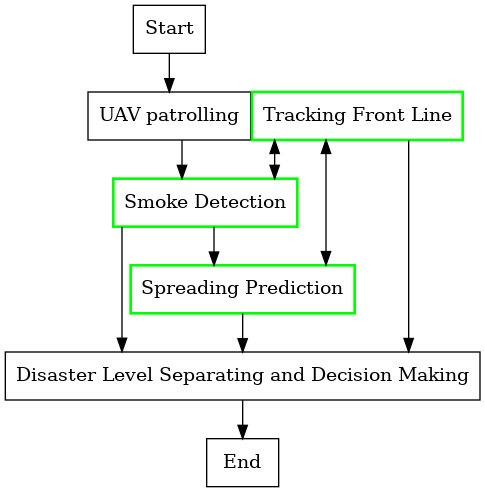
\includegraphics[width=60mm,height=60mm]{figs/arrangement.png}
    \caption{Main process of wildfire fighting using UAV}
    \label{fig:arrangement}
\end{figure}
Encouraged by so many excellent NN-based wildfire fighting strategies in recent years, this research is trying to design and develop a NN-based system with support of UAV and ground work station for early wildfire detection, prediction, and tracking with UAV. Fig.~\ref{fig:arrangement} is the brief structure of the wildfire detection and alarm system which is going to be build in this research. The main contributions could be induced in green boxed items, where they are detection, prediction and tracking. The reminder of the proposal of this research is structured as below:\par 
In Section 2, there are statements of related works and motivation of this research. Section 3 is the description and analysis of objective of this report. Some concepts of the proposed and preparing methodologies are placed in Section 4. Conclusions and potential future works are outlined in Section 5. Timeline and some of research process are illustrated in appendix.\par

\vspace{-0.3cm}

\section{Related Works and Motivation}
As analyzed in literature review before this report, traditional schemes for detecting wildfire early and analyzing wildfire actions are based on the features of wildfire smoke and flame. And, deep-neural-network-based (DNN-based) schemes focus more on the feature-learning processes in recent years. In this section, the state-of-art of NN-based wildfire detection and wildfire spreading predictions are studied.
% Fig.~\ref{fig:features} illustrated the commonly used features of smoke and flame for training these DNN models.
% \begin{figure}[ht]
%     \centering
%     \begin{subfigure}{.58\linewidth}
%     \centering
%         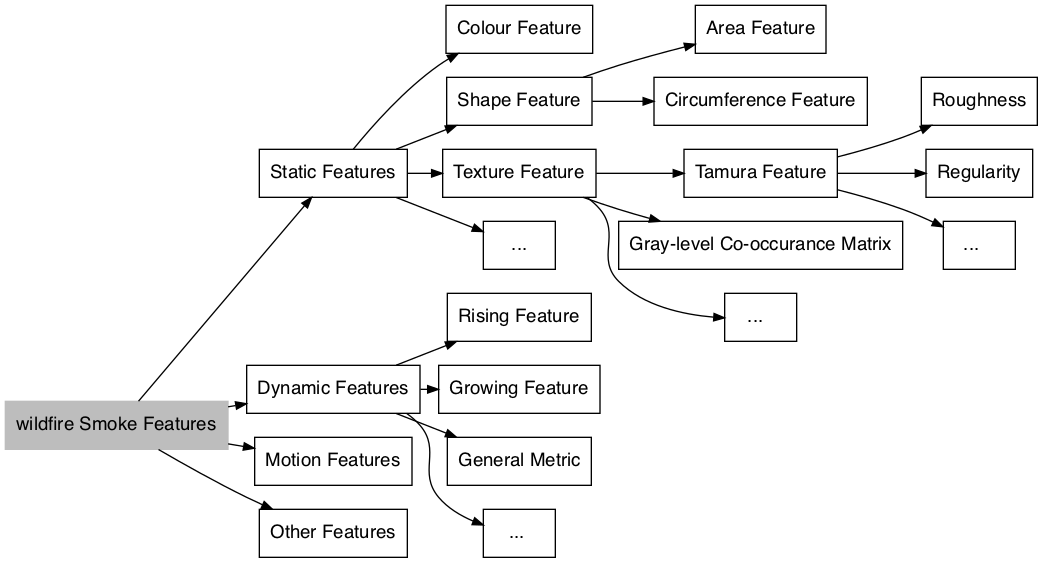
\includegraphics[height = 55mm]{figs/figuresmokefeatures.png}
%         \caption{}
%     \end{subfigure}
%     \begin{subfigure}{.4\linewidth}
%     \centering
%         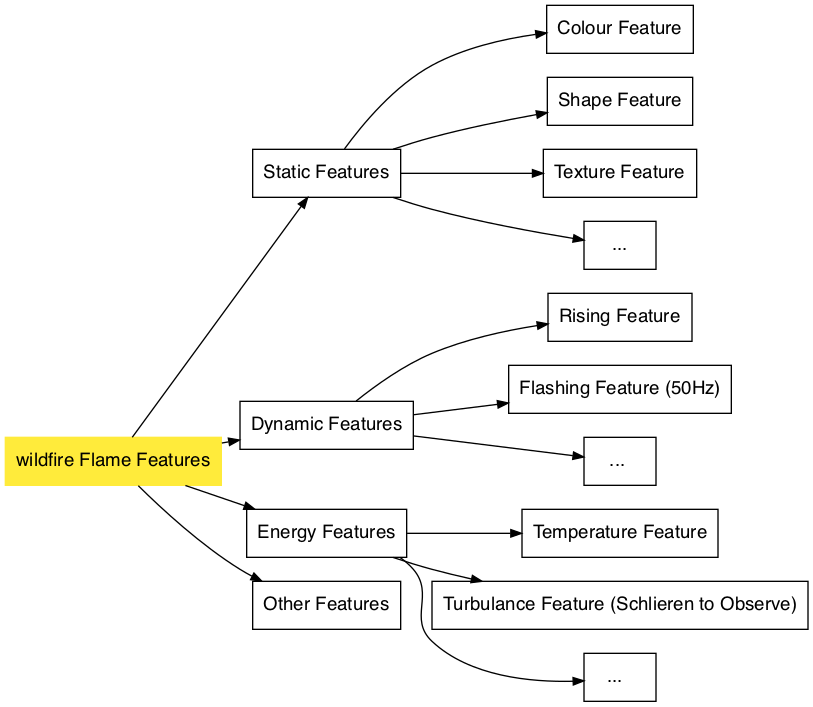
\includegraphics[height = 61mm]{figs/figureflamefeatures.png}
%         \caption{}
%     \end{subfigure}
%     \caption{Commonly applied smoke features and flame features for image-processing-based wildfire detection and analysis. (a) The commonly used smoke features for wildfire detection. (b) The commonly used flame features for wildfire detection.}
%     \label{fig:features}
% \end{figure}
\par
\subsection{NN-based Wildfire Detection Schemes}
For wildfire detection and other recognition tasks, DNNs are higher recommended. Generally, deep networks ensured higher level features could be extracted and better generalized. Also, with the help of transfer learning, it is easier to build segmentation network models for wildfire detection. U-net, one typical fully connected network (FCN) is widely accepted and applied in wildfire detection \cite{li2019detection, park2020wildfire, he2016deep, huang2017densely, mommert2020characterization}. There are also region-based convolutional network (R-CNN) \cite{lee2019deep} and recurrent neural network (RNN) \cite{jeong2020light} models could finish sequence-to-sequence analysis of wildfire data to detect smoke or flame.\par
However, in the most recent research, it is found that layers in these models are more computational complex. Because of the demand of early detection. The networks are often considered to be deployed on-board for UAV or UAVs. Saving the computing resource and simplifying the structure of networks are very challenging.\par 
Under such situation, light network models are studied. In \cite{peng2019real}, depthwise seperable convolution and SqueezeNet are considered to build blocks called fire model to detect wildfire. Based on fire models, a light U-net is proposed \cite{zhang2021att} to share parameters and save computing resources. on the other hand, attention mechanism is demonstrated that they could keep more deeper information in the down sampling process and decreased false positive detection \cite{oktay2018attention}. Also, it is found that attention layers is lower computational complexity by comparing with convolutional layer \cite{vaswani2017attention} in the research of Transformer. Vision transformer (ViT) model demonstrated that attention mechanism performed well in higher-resolution tasks \cite{zhang2018image}.\par
However, the application of attention mechanism also has its challenges. For example, for sequence data set, attention could not capture the order information, which limited the attention to learn partial information. These researches motivated the design and implementation to optimize the encoder-decoder structured model or models combining with attention mechanism for wildfire detection to save more computational resource and perform more meticulous and accurate segmentation.
\subsection{Wildfire Prediction Schemes}
After detecting the wildfire, it is also important to understand the dynamics and actions of wildfire, which motivated the study of wildfire spreading models. For a long period, wildfire spreading prediction are mainly rely on two typical numerical model:\par
The fist one is based on physical modeling accounting for various physical and chemical phenomena. This kind of model contains computational-fluid-dynamics (CFD) \cite{mueller2014large} which could describe the spreading progress with more details. However, its performance on real fire still need more discussion because of high computational cost and the environmental complexity.\par
The second one is the mathematical model which based on empirical model of rate of spread (RoS). As illustrated in \cite{alexandridis2008cellular}, mathematical growth prediction models is an acceptable description for wildfire spreading. Similar as fire area simulator (FARSITE) \cite{finney1999farsite}, a type consists of models based on continuous plane assumed the fire spreads in a continuous landscape and solving a system of partial differential equations is considered as the solution of these models\cite{richards1995general}. A computationally faster type consists of the models based on grid \cite{pastor2003mathematical}. Typically, there are Cellular Automata (CA) \cite{trunfio2004predicting} and Bond-Percolation method. Compared with Bond-percolation method, CA solved its problem of describing the dynamics of the fire spread. There are also some other types of models, such as the fuzzy or neural based ones \cite{vakalis2004gis1,vakalis2004gis2}.\par
\begin{figure}[ht]
    \centering
    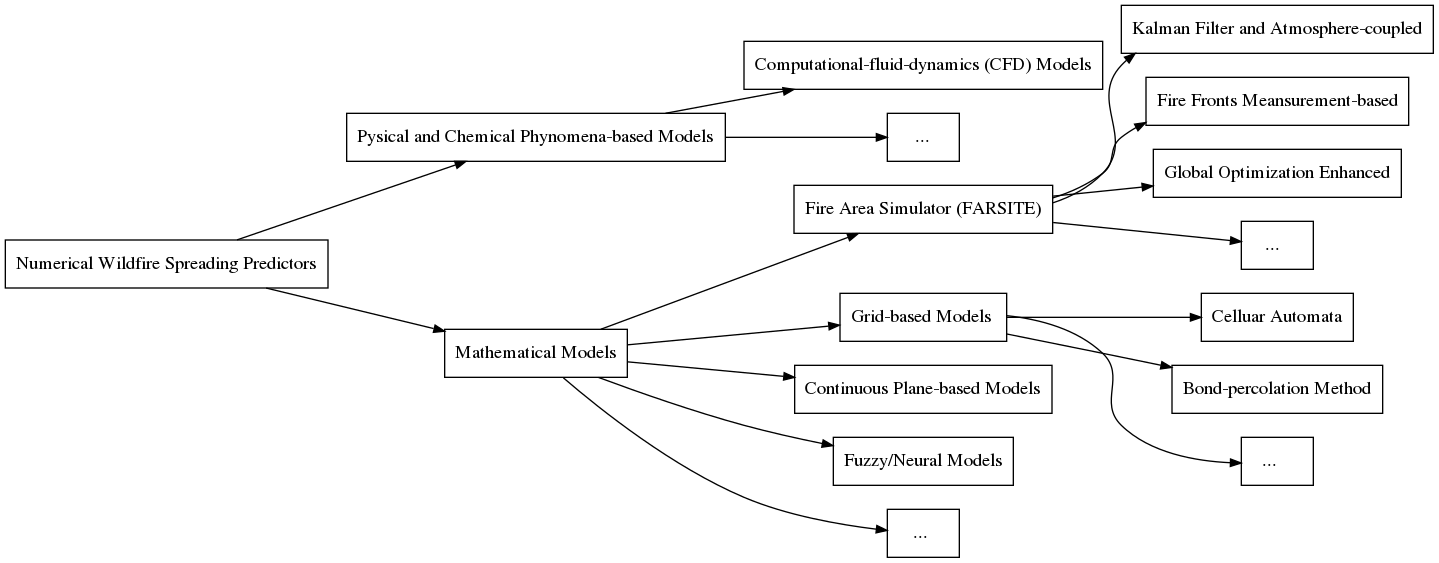
\includegraphics[height=68mm]{figs/figurepredictionmodel.png}
    \caption{Main schemes for predicting the wildfire spread}
    \label{fig:spreadmodel}
\end{figure}
Generally, data-driven schemes could be applied for improving the accuracy of locating fire fronts and reduce the simulation uncertainty. In the review \cite{zhai2020learning}, Kalman filter, Lagrangian particle, Huygens principle and level-set method are mentioned to predict the fire front based on the real-time RoS measurement.
The aforementioned schemes could be illustrated in Fig.~\ref{fig:spreadmodel}. In recent years, it is found that data collected from geographic information system (GIS) and data augmentation with some NN models are also helpful in building these models. For example, the performance of FireCast of 2D-CNN \cite{radke2019firecast} and LSTM \cite{huot2020deep} both encouraging.\par 
However, these models often work for a relatively large time step (hours or days) \cite{burge2020convolutional}. The complex forest environment might change rapidly during the early fire period. To improve the accuracy and prediction speed need more investigation and demonstration. Such objectives motivated that the application of probabilistic models \cite{pimont2021prediction}, attention mechanism \cite{vaswani2021scaling}, and some popular DNN models to be applied.\par
\subsection{Vision-based Wildfire Tracking Schemes}
The prediction schemes mentioned above could be treated as a kind of auto-regressive processes. However, they are nearly to predict the wildfire scar, where the vegetation are already burnt, improving the accuracy of the fire front prediction is much more challenging for such indirect schemes by considering the wind-slope and other interacting factors. The accuracy and sensitiveness limitations are considered. Therefore, remote-sensing (equipped UAV) supported fire fronts tracking is thought about to ensure the predictions and monitoring of suspected wildfire areas.\par
Commonly, in forest fire management, visual object tracking (VOT) is the most efficient tracking scheme, VOT is studied in this research. VOT could be evaluated through OTB50 or OTB100 benchmarks \cite{wu2013online}. The mainly applied VOT scheme consists of traditional 
% 迭代模型
generative model (GM),
% 判别模型
discriminative model (DM),
% deep learning model
and the DNN-based model getting hot in recent years. 
Commonly, GM build the objective model or extract the objective features at first, then it would search the similar features in the coming frames, and iterated to locate the tracking target. However, the background information and the randomness and multiple shape changing of target are not efficiently used when it is used in environment where it is lower resolution, brightness changing, which limited its accuracy in wildfire management. Compared with GM, DM performs better in mean frame per second (FPS) and mean precision. DM extracts and locates the target in local frame by comparing the different information of target and background. Related filters and some machine learning based classifiers are being applied as DM for VOT. Also, there is DNN-based model, which is different from GM and DM \cite{krebs2017survey}. These main schemes could be illustrated in Fig.~\ref{fig:figuretrackingmodel}.
\begin{figure}[ht]
    \centering
    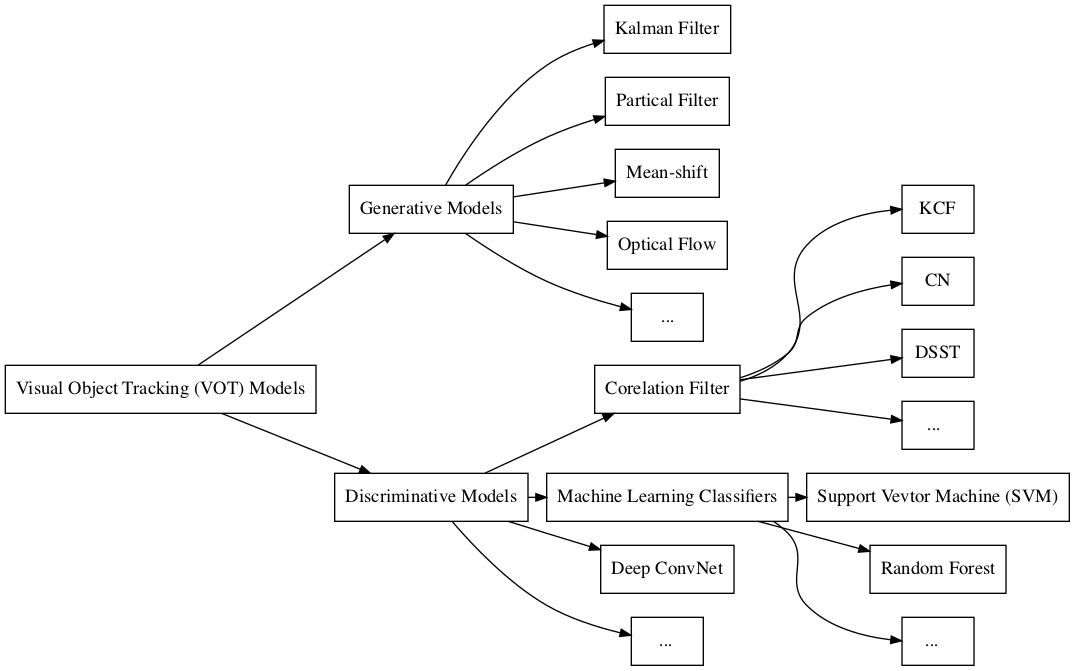
\includegraphics[height=80mm]{figs/figuretrackingmodel.png}
    \caption{Main schemes could be applied for tracking fire fronts}
    \label{fig:figuretrackingmodel}
\end{figure}
\par
With the support of VOT, UAV or UAVs could track or avoid the smoke and flame area and give fire fighters more information in wildfire management tasks. The 
\vspace{-0.3cm}

\section{Scope and Objectives}
The mainly focus goals of this research contain two parts: The first part is to use DNN-based models to save computational resources when detecting and predicting the wildfire. The second part is to design the tracking scheme for UAV or UAVs to track the suspected burning area in forest. Therefore, the proposed research plan is organized around the following objectives:\par
\begin{itemize}
    \item \textit{Detection and segmentation objective:} Considering DNN model as an efficient wildfire segmentation scheme, design and develop the detection network structure so that the parameters could be used more efficient.
    \item \textit{Deployment objective:} Design and develop light network structure so that it could be deployed on-board with UAV or UAVs, so that the path planning algorithm and detection scheme could work on-board with acceptable FPS at mean time.
    \item \textit{Optimization objective:} Develop and test the attention mechanism in segmentation networks to share the parameters. Compared with convolutional layers, it is found that attention layers are lower computational complex.
    \item \textit{Prediction objective:} Based on FARSITE and cellular model, build a wildfire spreading model which could predict the wildfire under impacts of wind and slope with acceptable accuracy.
    \item \textit{Coverage and tracking objective:} Design the tracker for UAV which could track wildfire spreading in safe and efficient distance.   
\end{itemize}\par
The proposed research in brief is expected to deploy the detection model on both UAV and ground work station. Considering the uncertain factors in forest environment, image restoration, prediction scheme, and UAV tracking should also be applied to support the detection. Because of the demand of early and accurate detection, DNNs is focused, as designed and developed for image restoration, detection, prediction and tracking. These strategies in this research and work are going to be demonstrated and verified through simulation and experiments through ground station computer and DJI M300 quad-copter equipped with H20T infrared camera.



\section{Methodologies}
\subsection{U-net-based Wildfire Detection}
Considering the rapidly shape changing and blurred edge of smoke, U-net is advocated in this research because of its fantastic performance in medical image processing fields. With the original image information or the restored images from UAV in forest, U-net could be deployed for wildfire smoke or flame segmentation. The U-net structure could be illustrated in Fig.~\ref{fig:figureUnetmodel}.
\begin{figure}[ht]
    \centering
    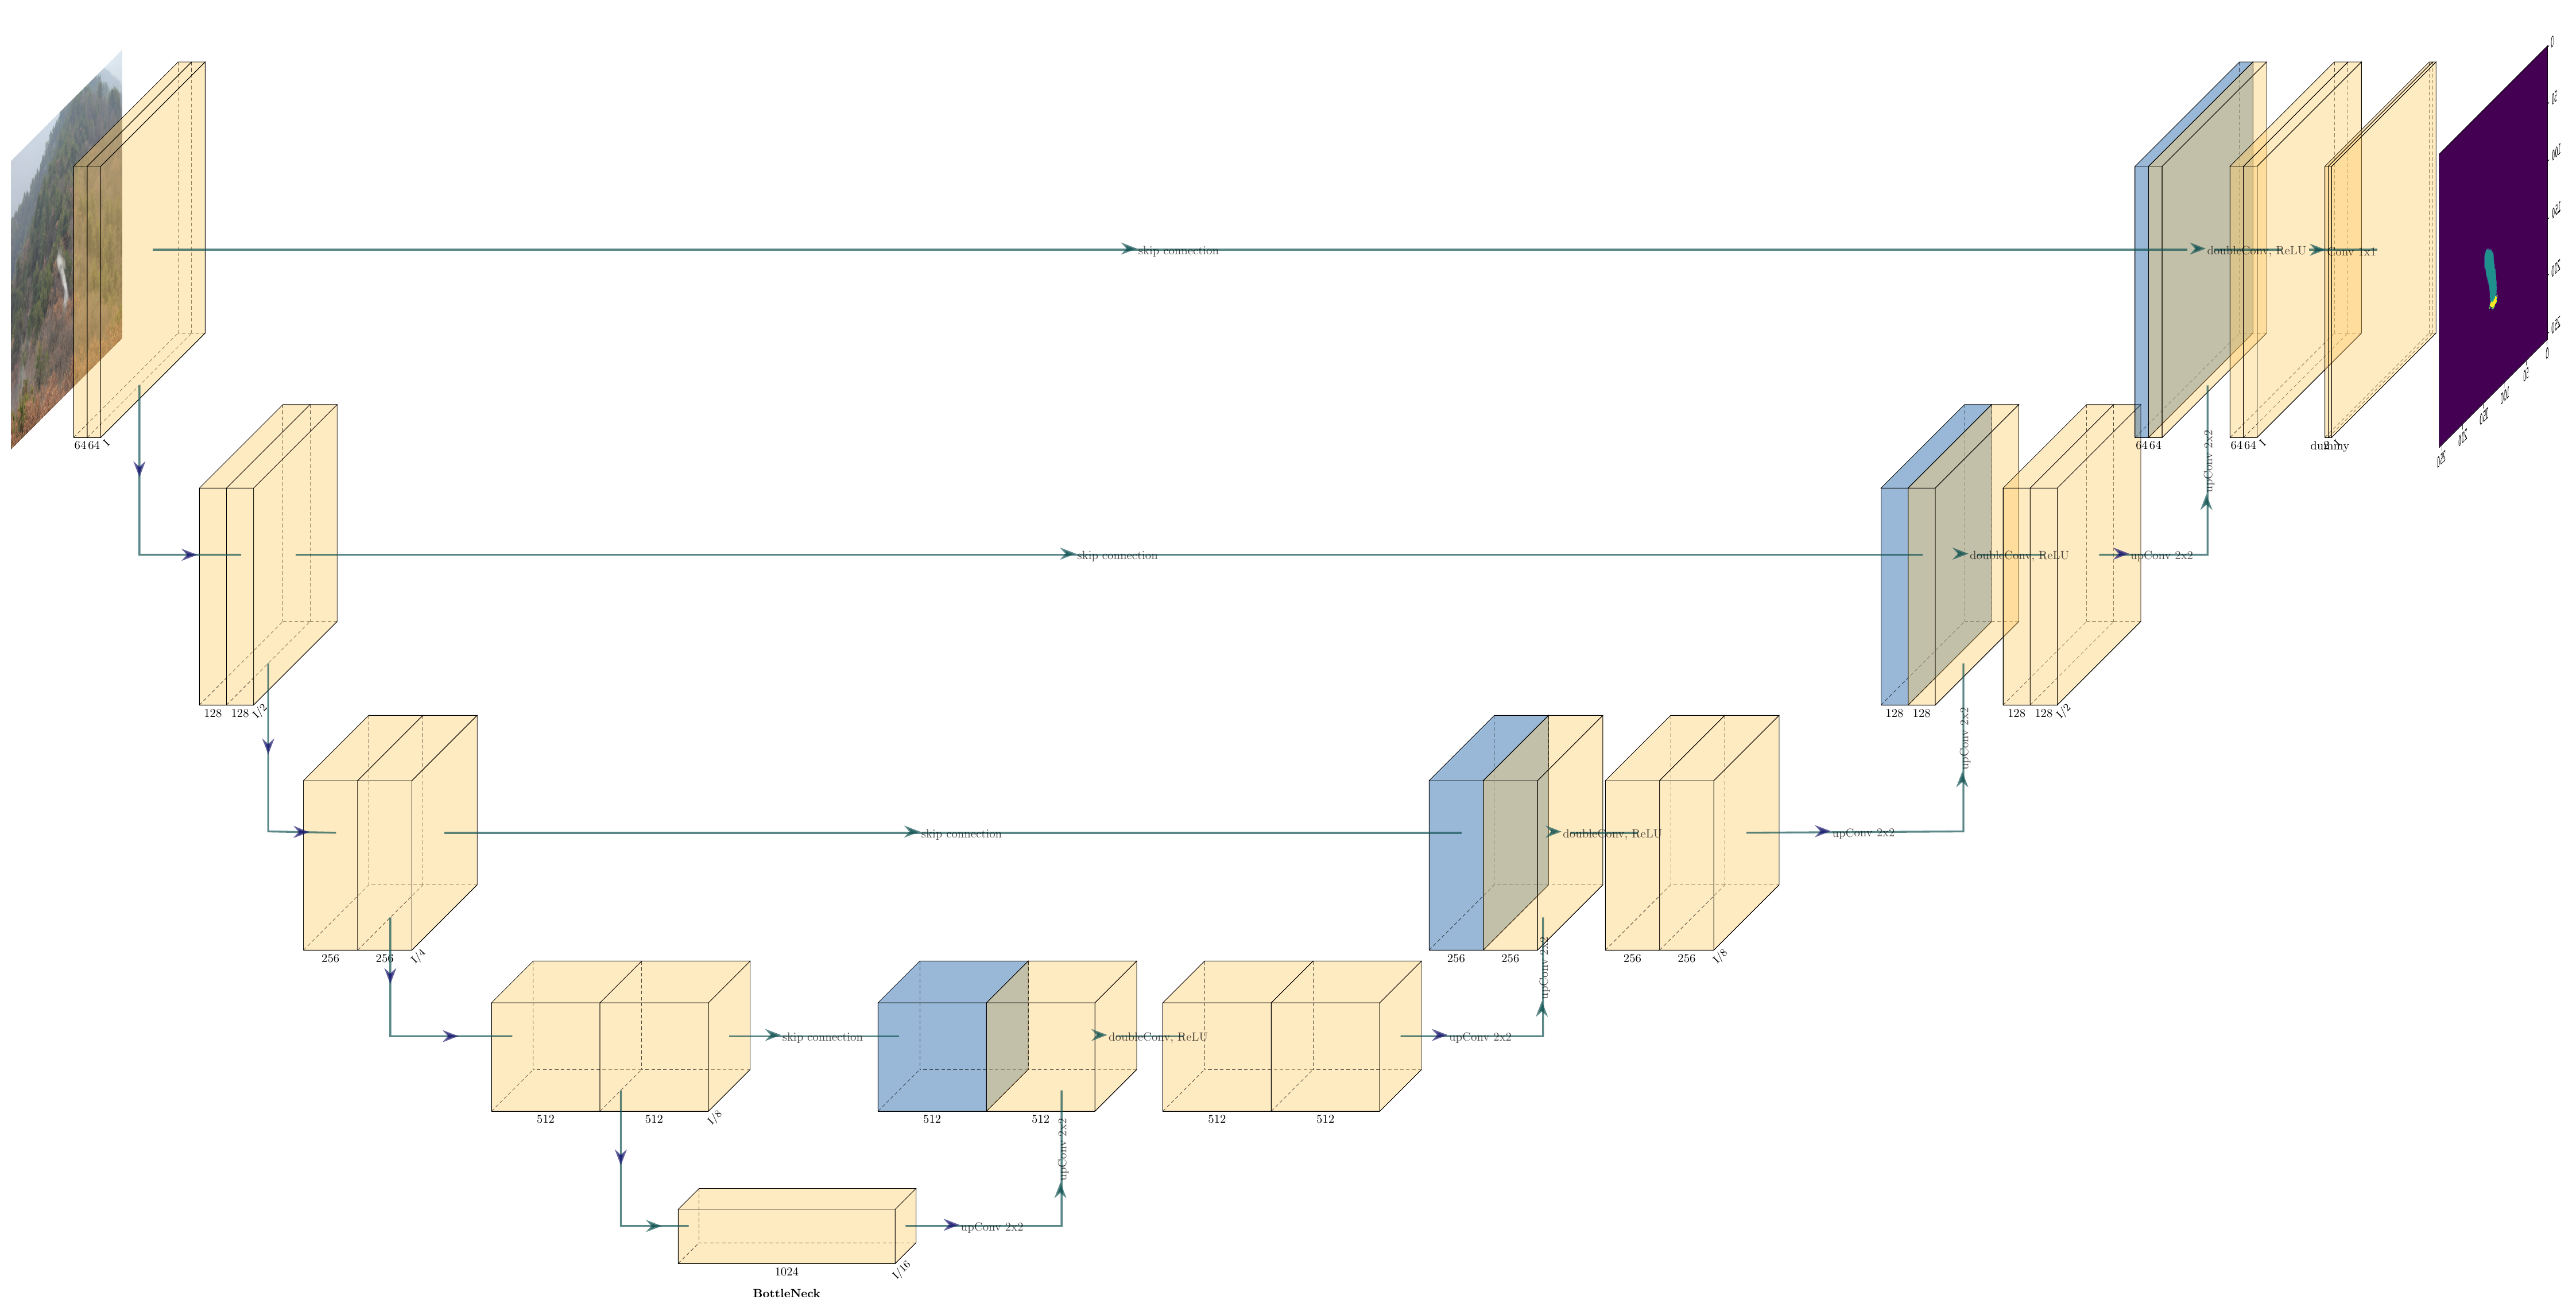
\includegraphics[height=60mm]{figs/figureUnetmodel.png}
    \caption{Brief structure of the U-net deployed on DJI M300 for the first time experiment}
    \label{fig:figureUnetmodel}
\end{figure}\par
The structure shown in Fig.~\ref{fig:figureUnetmodel} is the one which based on ResNet18 and the first time experiment demonstrated that it could be deployed on-board with the support of tensor2trt to get FPS of 5 as dealing with original images. However, the segmentation accuracy still need to be improved and the size of this model could be decreased when using the concept of SqueezeNet. At ground work station, the deployment environment is not that serious as on-board, but the segmentation accuracy should be higher than on-board ones. Therefore, higher level residual networks could also be considered to build a U-net for wildfire smoke and flame segmentation. These apply-able network structures are illustrated in Table.~\ref{table: fcnforunet}.
\begin{table}[!ht]
    \centering
    \caption{Residual network structures for building the U-net for wildfire detection}
    \label{table: fcnforunet}
        \resizebox{\textwidth}{!}{
        \begin{tabular}{c c c c c c c}
        \toprule
        Layers &
        Output &
        18-layers&
        34-layers&
        50-layers&
        101-layers&
        152-layers\\
        \midrule
        \rowcolor{mygray}
        Conv1 &
        $112\times 112$&
        \multicolumn{5}{c}{
        \text{kernel size} = $7\times7$, \text{out channel} = 64, \text{stride} = 2, \text{padding} = 3
        } \\
        \rowcolor{mygray}
        Pool1 &
        $112\times 112$&
        \multicolumn{5}{c}{
        \text{kernel size} = $3\times3$, \text{type} = \text{max pool}, \text{stride} = 2
        }\\
        Conv2x &
        $56\times 56$&
        \left[
        \begin{array}{c}
            3\times 3, 64\\ 3\times 3, 64
        \end{array}
        \right] \times 2 &
        \left[
        \begin{array}{c}
            3\times 3, 64 \\ 3\times 3, 64
        \end{array}
        \right] \times 3 &
        \left[
        \begin{array}{c}
            1\times 1, 64 \\ 3\times 3, 64\\ 1\times 1, 256\\
        \end{array}
        \right] \times 3 &
        \left[
        \begin{array}{c}
            1\times 1, 64 \\ 3\times 3, 64\\ 1\times 1, 256
        \end{array}
        \right] \times 3 &
        \left[
        \begin{array}{c}
            1\times 1, 64 \\ 3\times 3, 64\\ 1\times 1, 256
        \end{array}
        \right] \times 3\\
        
        \rowcolor{mygray}
        Conv3x&
        28\times 28&
        \left[
        \begin{array}{c}
             3\times 3, 128\\ 3\times 3, 128
        \end{array}
        \right] \times 2 &
        \left[
        \begin{array}{c}
            3\times 3, 128 \\ 3\times 3, 128
        \end{array}
        \right] \times 4 &
        \left[
        \begin{array}{c}
            1\times 1, 128 \\ 3\times 3, 128\\ 1\times 1, 512
        \end{array}
        \right] \times 4 &
        \left[
        \begin{array}{c}
            1\times 1, 128 \\ 3\times 3, 128\\ 1\times 1, 512
        \end{array}
        \right] \times 4 &
        \left[
        \begin{array}{c}
            1\times 1, 128 \\ 3\times 3, 128\\ 1\times 1, 512
        \end{array}
        \right] \times 8 &\\
        Conv4x &
        14\times14&
        \left[
        \begin{array}{c}
            3\times 3, 256 \\ 3\times 3, 256\\
        \end{array}
        \right] \times 2 &
        \left[
        \begin{array}{c}
            3\times 3, 256 \\ 3\times 3, 256\\
        \end{array}
        \right] \times 6 &
        \left[
        \begin{array}{c}
            1\times 1, 256 \\ 3\times 3, 256\\ 1\times 1, 1024
        \end{array}
        \right] \times 6 &
        \left[
        \begin{array}{c}
            1\times 1, 256 \\ 3\times 3, 256\\ 1\times 1, 1024
        \end{array}
        \right] \times 23 &
        \left[
        \begin{array}{c}
            1\times 1, 256 \\ 3\times 3, 256\\ 1\times 1, 1024
        \end{array}
        \right] \times 36 &\\
        \rowcolor{mygray}
        Conv5x&
        7\times7&
        \left[
        \begin{array}{c}
            3\times 3, 512 \\ 3\times 3, 512
        \end{array}
        \right] \times 2 &
        \left[
        \begin{array}{c}
            3\times 3, 512 \\ 3\times 3, 512
        \end{array}
        \right] \times 3 &
        \left[
        \begin{array}{c}
            1\times 1, 512 \\ 3\times 3, 512\\ 1\times 1, 2048
        \end{array}
        \right] \times 3 &
        \left[
        \begin{array}{c}
            1\times 1, 512 \\ 3\times 3, 512\\ 1\times 1, 2048
        \end{array}
        \right] \times 3 &
        \left[
        \begin{array}{c}
            1\times 1, 512 \\ 3\times 3, 512\\ 1\times 1, 2048
        \end{array}
        \right] \times 3\\
        \bottomrule
        \end{tabular}}
\end{table}
\subsection{Squeeze Model}
To deploy the U-net on-board with less computational resource demands, the squeeze model is consider for developing the ResNet18-based U-net into a light model. Attention mechanism is also able to be developed to design attention gate at the skip connection parts of U-net to filter higher value features before up-sampling parts to increase the feature learning efficiency.\par
On the other hand, attention mechanism could not only be applied to develop the U-net for wildfire detection. It could also be helpful in building the NN-based prediction model for the fire fronts spreading. Such concept is also stated at the conclusion part of \cite{peng2019real}. Therefore, the squeeze model and attention mechanism are going to be described as follow.
\subsubsection{Squeeze Model}
Fig.~\ref{fig:figureSqueezemodel} shows the brief structure of the squeeze and unsqueeze model.

\subsubsection{Attention Mechanism}

\subsection{GAN-based Wildfire Image Restoration}
Considering the signal missing and disturbance as UAV capturing image information in wide forest environment. Generative adversarial network (GAN)-based image restoration is going to be designed. GAN could be separate into two parts: generator ($G$) and discriminator ($D$). The generating continues until the discriminator could not distinguish which is the target or which is the generated image, it is considered converged.\par
It should be noticed that, such strategy should only be applied in very serious forest environment and extreme situation. Because the GAN should be deployed on-board, where the computation resource distribution will be very challenging as other schemes are working to support the wildfire detection. And strictly, the restored information are not the real original information, there is risk that the restored image might misleading the segmentation of smoke edge.
Commonly, the GAN structure could be illustrated in Fig.~\ref{fig:figureGANmodel}.
\begin{figure}[ht]
    \centering
    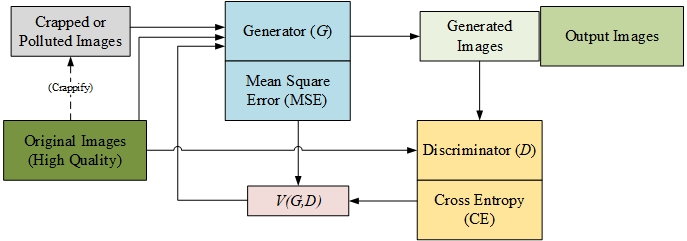
\includegraphics[height=40mm]{figs/figureGANmodel.jpg}
    \caption{Brief GAN structure as training process}
    \label{fig:figureGANmodel}
\end{figure}
It could be considered that, GAN is to balance the loss of $G$ and $D$. Mean squared error (MSE) could be applied as the main loss function of GAN. In the training process, MSE is to compare the pixel values of generated image and high quality image, it can be written in a form of Eq.~\ref{eq: MSE}.
\begin{equation}
\text{MSE}(y, \hat y) =
\frac{\sum_{i=0}^N (y_i-\hat y_i)^2}{N}
\label{eq: MSE}
\end{equation}
Value function $V(G, D)$ could be applied as Eq.~\ref{eq: valueloss} to describe the balance process of GAN.
\begin{equation}
\min_G\max_D V(G,D)=
\mathbf{E}_{x~p_{data}{x}}[\log D(x)]+
\mathbf{E}_{z~p_z{z}}[log(1-D(G(z)))]
\label{eq: valueloss}
\end{equation}
\subsection{Cellular Model for Wildfire Prediction}
\subsection{VOT-based Wildfire Tracking}







\section{Timeline} \label{timeline}
The following Table~\ref{table:timeline} outlines the process for accomplishing the objectives of the PhD study.
\begin{table}[!ht]
    \centering
    \caption{Timelines for PhD study}
    \label{table:timeline}
        \resizebox{\textwidth}{!}
        {
        \begin{tabular}{c c c c c c c c c c c c c}
        \toprule
        \multirow{2}{6cm}{
        \centering
        Main Tasks
        }&
        \multicolumn{3}{c}{
        2018-2019
        }&
        \multicolumn{3}{c}{
        2019-2020
        } &
        \multicolumn{3}{c}{
        2020-2021
        } &
        \multicolumn{3}{c}{
        2021-2022
        }\\
        &
        \cellcolor{mygray}W& \cellcolor{mygray}S& \cellcolor{mygray}F&
        W& S& F&
        \cellcolor{mygray}W& \cellcolor{mygray}S& \cellcolor{mygray}F&
        W& S& F\\
        \hline
        % \rowcolor{mygray}
        Course Study&
        \cellcolor{mygray}$>$& \cellcolor{mygray}$>$& \cellcolor{mygray}$>$&
        & & & 
        \cellcolor{mygray}& \cellcolor{mygray}& \cellcolor{mygray}&
        & & \\
        
        Literature Review&
        \cellcolor{mygray}$>$& \cellcolor{mygray}$>$& \cellcolor{mygray}$>$&
        $>$& $>$& $>$& 
        \cellcolor{mygray}$>$& \cellcolor{mygray}$>$& \cellcolor{mygray}$>$&
        & & \\
        
        % \rowcolor{mygray}
        Comprehensive Exam &
        \cellcolor{mygray}& \cellcolor{mygray}& \cellcolor{mygray}&
        & & &
        \cellcolor{mygray}& \cellcolor{mygray}$>$& \cellcolor{mygray}&
        & & \\
        
        ResNet for Wildfire Detection&
        \cellcolor{mygray}& \cellcolor{mygray}& \cellcolor{mygray}&
        $>$& $>$& $>$&
        \cellcolor{mygray}& \cellcolor{mygray}& \cellcolor{mygray}&
        & & \\
        
        % \rowcolor{mygray}
        GAN for Image Restoration&
        \cellcolor{mygray}& \cellcolor{mygray}& \cellcolor{mygray}&
        & $>$& $>$& 
        \cellcolor{mygray}$>$& \cellcolor{mygray}& \cellcolor{mygray}&
        & &  \\
        
        Attention Mechanism&
        \cellcolor{mygray}& \cellcolor{mygray}& \cellcolor{mygray}&
        $>$& $>$& $>$&
        \cellcolor{mygray}$>$& \cellcolor{mygray}$>$& \cellcolor{mygray}$>$&
        $>$& $>$& $>$\\
        
        % \rowcolor{mygray}
        Develop for On-board Deployment&
        \cellcolor{mygray}& \cellcolor{mygray}& \cellcolor{mygray}&
        & & &
        \cellcolor{mygray}& \cellcolor{mygray}& \cellcolor{mygray}$>$&
        $>$& & \\

        DNN Enhanced Cellular for Wildfire Prediction&
        \cellcolor{mygray}& \cellcolor{mygray}& \cellcolor{mygray}&
        & $>$& $>$&
        \cellcolor{mygray}$>$& \cellcolor{mygray}$>$& \cellcolor{mygray}$>$&
        $>$& & \\
        
        % \rowcolor{mygray}
        Vision of Tracking for Fire Fronts with UAV(UAVs)&
        \cellcolor{mygray}& \cellcolor{mygray}& \cellcolor{mygray}&
        & & &
        \cellcolor{mygray}$>$& \cellcolor{mygray}$>$& \cellcolor{mygray}$>$&
        $>$& & \\
        
        Publications&
        \cellcolor{mygray}& \cellcolor{mygray}& \cellcolor{mygray}&
        $>$& $>$& $>$&
        \cellcolor{mygray}$>$& \cellcolor{mygray}& \cellcolor{mygray}$>$&
        $>$& $>$& $>$\\
        \bottomrule
        
        
        \end{tabular}
        }
\end{table}

\section{Anticipated Significance of the Work}
The merits of this proposed research can be reflected by an anticipated significant contribution to the concept of smart forestry, especially the UAV-based forest firefighting. It is an essential work to improve the wildfire detection and location accuracy  with UAV during the early fire period. The main idea of this work is to save the limited computational resource on-board and decrease the false positive in wildfire discovering stage.
The results of the proposed work would be published in journal and conference publications. Some preliminary results of the proposed research have been presented  in the following conference:






\newpage
\small
\bibliographystyle{IEEEtran}
\bibliography{reference}

\newpage
\pagenumbering{Roman}
\section{Appendix: Process to Date}
With respect to the presented timeline (Table~\ref{table:timeline}) in Section.~\ref{timeline}, this section provides a brief review of the process to date of the PhD thesis work. The works focused on the objectives of: wildfire image restoration, wildfire detection, and fire fronts prediction. They are separately stated as follow.
\subsection{Wildfire Image Restoration}
To develop the robustness of GAN for wildfire image restoration, a feature loss is proposed to improve the original confusion loss of U-net-based GAN. The simulation programmings of the restoration are illustrated in Table~\ref{table:GANprogram}.
\begin{table}[ht]
\caption{The simulation basement of proposed feature loss GAN for wildfire image restoration}
\label{table:GANprogram}
    \centering
    \small
    \begin{tabular}{c c}
    \toprule
        Names & Illustrations\\
        \hline
        \rowcolor{mygray}
        Platform & Google Cloud Platform (GCP)\\
        Framework &  Pytorch, Fastai\\
        \rowcolor{mygray}
        GPU & nvidia-tesla-t4\\
        GAN Structure & ResNet-based U-net\\
        \rowcolor{mygray}
        Feature Loss Network& VGG16-based U-net\\
        Dataset Resource& Google Images \\
    \bottomrule
    \end{tabular}
\end{table}\par
The training process losses are shown in Fig.~\ref{fig:GANlosscompare}. There is an obvious jumping of validation loss as the entire U-net structure of GAN is unfreezed, which shows the jumping out of local minimum.
\begin{figure}[ht]
\centering
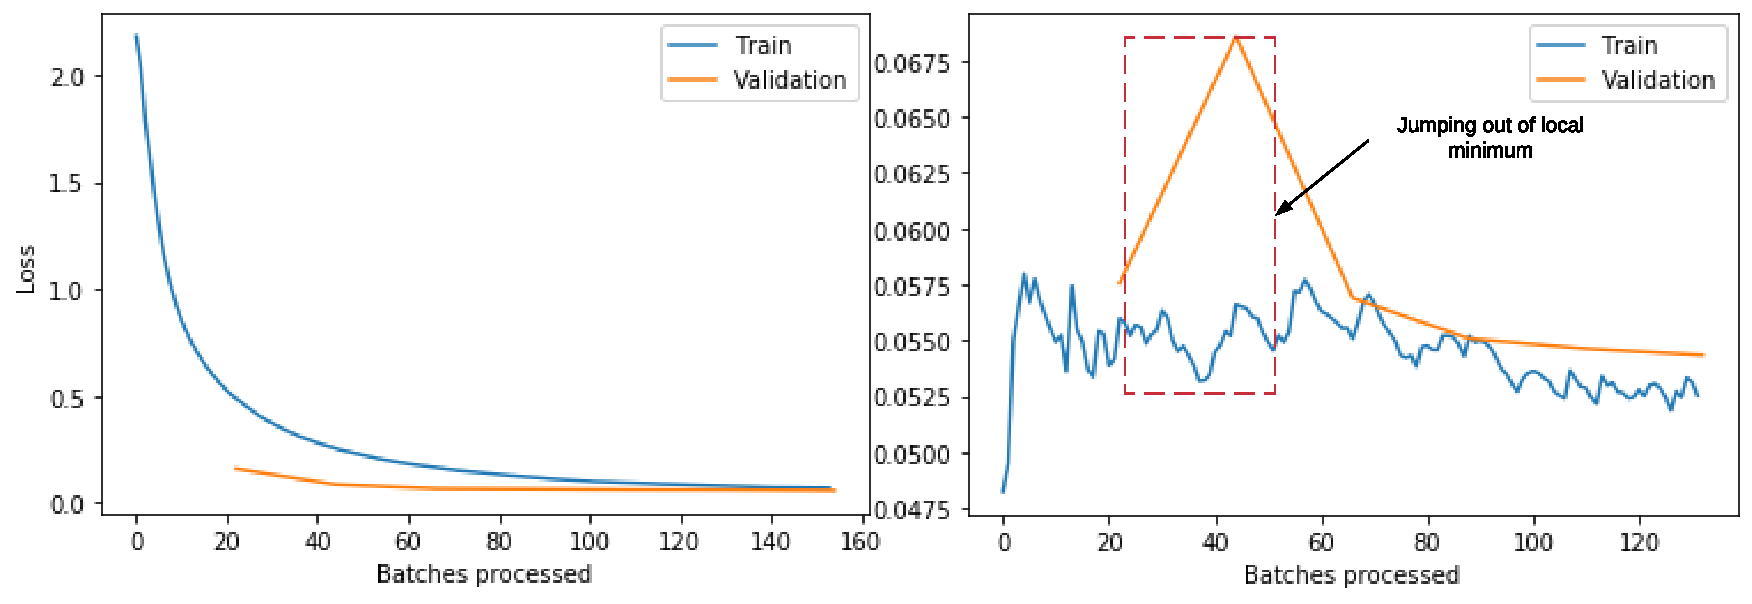
\includegraphics[height=50mm]{figs/GANlosscompare.pdf}
\caption{U-net training loss and validation loss changing. Left: Freeze encoder part of U-net; Right: Unfreezed encoder-decoder U-net. It seems over trained but jumped out of local minimum.}
\label{fig:GANlosscompare}
\end{figure}\par
 The final restoration performance is shown in Fig.~\ref{fig:GANoutcompare} by comparing with the single VGG16-based GAN, the proposed model shows higher robustness.
\begin{figure}[ht]
\centering
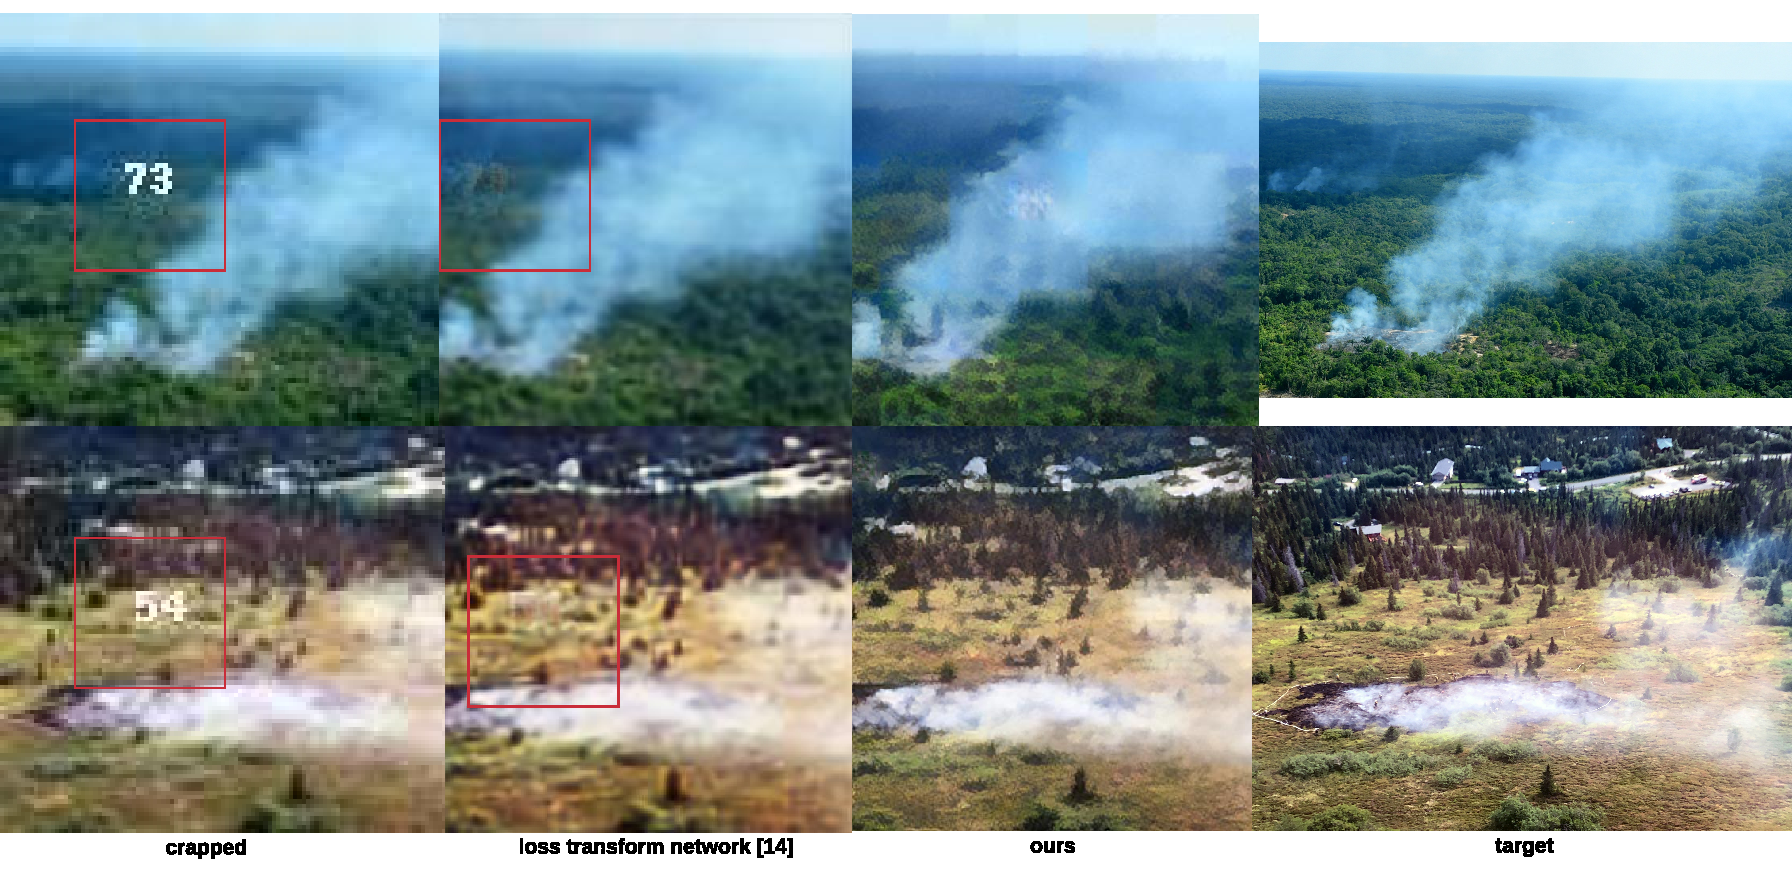
\includegraphics[height=60mm]{figs/GANoutcompare.pdf}
\caption{The GAN restoration output. Left column: Crapped images, number marks are randomly added as disturbance at random location in images, higher number order means the image is randomly crapped more. Mid-left column: Restoration results of feature loss network. Mid-right column: Restoration results of proposed loss GAN. Right column: Original images (targets).}
\label{fig:GANoutcompare}
\end{figure}\par

\subsection{Wildfire Classification}
The wildfire images classification is designed for UAV or UAVs to discriminate whether there suspected smoke or flame is contained in the image. This program is working before the segmentation on-board. Because the segmentation program might cause more computation and energy cost of on-board computer and battery. The designed classification contains ResNet34 based classifier and developed attention mechanism-based classifier. Their simulation basement are stated in Table.~\ref{table:classprogram}, and their classification results are shown as follow in Fig.~\ref{fig:classresnetattention}.
\begin{table}[ht]
\centering
\caption{The simulation basement of proposed ResNet34-based and Attention mechanism-based wildfire classifiers}
\label{table:classprogram}
    \small
    \begin{tabular}{c c c}
    \toprule
        Names & ResNet34-based Classifier &  Attention-based Classifier\\
        \hline
        Dataset Source& \multicolumn{2}{c}{Google Images, Kaggle Dataset}\\
        \rowcolor{mygray}
        Platform & \multicolumn{2}{c}{
        Personal Computer}\\
        Framework &  \multicolumn{2}{c}{Pytorch, Fastai}\\
        \rowcolor{mygray}
        CPU & \multicolumn{2}{c}{Intel-i7-4790K}\\
        \rowcolor{mygray}
        GPU & Nvidia-GTX-1060 & Nvidia-GTX-1660\\
        Pre-Training & False & ImageNet\\
    \bottomrule
    \end{tabular}
\end{table}
\begin{figure}[ht]
\centering
    \begin{subfigure}{.3\linewidth}
    \centering
        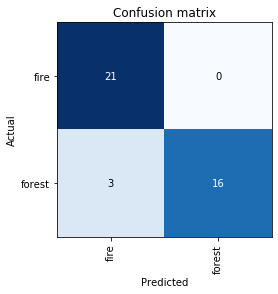
\includegraphics[width=50mm]{figs/classrensnet.png}
        \caption{}
    \end{subfigure}
    \begin{subfigure}{.3\linewidth}
    \centering
        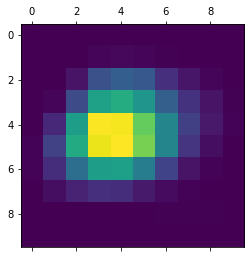
\includegraphics[width=50mm]{figs/classattention.png}
        \caption{}
    \end{subfigure}
    \begin{subfigure}{.3\linewidth}
    \centering
        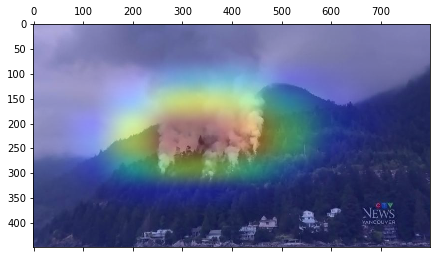
\includegraphics[width=50mm,height=50mm]{figs/classattention2.png}
        \caption{}
    \end{subfigure}
    \caption{\small Classification results of designed classifiers. (a) The confusion matrix of ResNet34-based wildfire classification. (b) The result heat-map of Attention-based wildfire classification. (c) The mixed heat-map mask and original image.}
    \label{fig:classresnetattention}
\end{figure}\par

\subsection{Wildfire Segmentation}
When the image is demonstrated as a wildfire image, it will be send into the segmentation program part so that the wildfire detection accuracy could be increased and the suspected fire point could be located more specific in the image.\par
The designed segmentation model on-board is based on pure U-net which has ResNet18 structure and the H20T infrared camera could be applied for directly detect the wildfire with appropriate threshold. The segmentation model on ground work station is based on ResNet34. For both the model on-board and on ground work station, attention mechanism and squeezed model should be designed to develop the model. The simulation and experience basement are separately illustrated in Table~\ref{table:segprogram}.
\begin{table}[ht]
\centering
\caption{The simulation basement of proposed on-board and ground segmentation model}
\label{table:segprogram}
    \small
    \begin{tabular}{c c c}
    \toprule
        Names & On-board Segmentation Model & Ground Segmentation Model\\
        \hline
        Dataset Source& \multicolumn{2}{c}{Kaggle Dataset, UAV Captured Experience Dataset}\\
        \rowcolor{mygray}
        Platform & YunGuan on-board computer with DJI M300 UAV& Personal Computer\\
        Framework &  DJI OSDK, ROS, Pytorch & Pytorch, Fastai\\
        \rowcolor{mygray}
        CPU & NAN& {Intel-i7-4790K}\\
        \rowcolor{mygray}
        GPU & Nvidia-Jetson & Nvidia-GTX-1660\\
        \rowcolor{mygray}
        Model Structure& ResNet18& ResNet34\\
        Pre-Training & ImageNet & ImageNet\\
    \bottomrule
    \end{tabular}
\end{table}
\par
As shown in Fig.~\ref{fig:segmentationGround} is the segmentation results of the proposed ResNet34-based U-net with attention gates in skip connection. The targets are frames randomly from a video captured by UAV, which is the dataset from Kaggle. The right column shows that the original designed model is sensitive, but with higher false positive. The developed model with attention gate sacrificed the sensitivity but decreased the false positive and increased accuracy.
\begin{figure}[ht]
    \centering
    \begin{subfigure}{.24\linewidth}
    \centering
        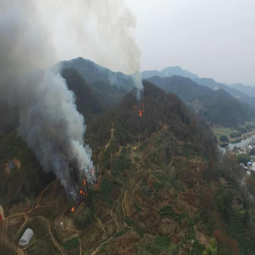
\includegraphics[width = 38mm]{figs/ain1.png}
    \end{subfigure}
    \begin{subfigure}{.24\linewidth}
    \centering
        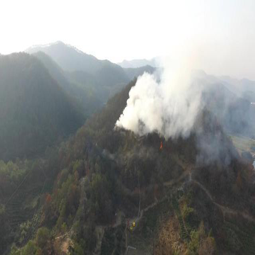
\includegraphics[width = 38mm]{figs/ain2.png}
    \end{subfigure}
        \begin{subfigure}{.24\linewidth}
    \centering
        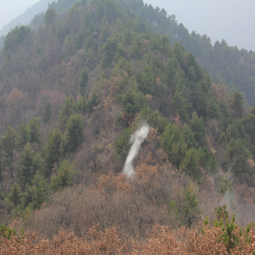
\includegraphics[width = 38mm]{figs/ain3.png}
    \end{subfigure}
    \begin{subfigure}{.24\linewidth}
    \centering
        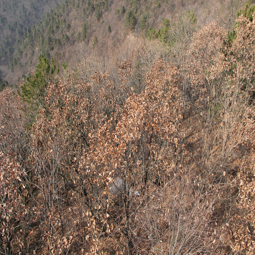
\includegraphics[width = 38mm]{figs/ain4.png}
    \end{subfigure}
        \begin{subfigure}{.24\linewidth}
    \centering
        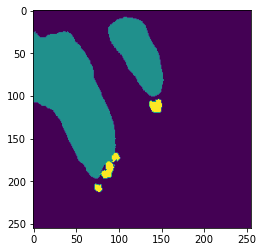
\includegraphics[width = 41mm]{figs/aunet1.png}
    \end{subfigure}
    \begin{subfigure}{.24\linewidth}
    \centering
        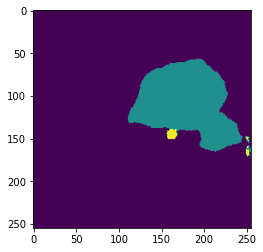
\includegraphics[width = 41mm]{figs/aunet2.png}
    \end{subfigure}
        \begin{subfigure}{.24\linewidth}
    \centering
        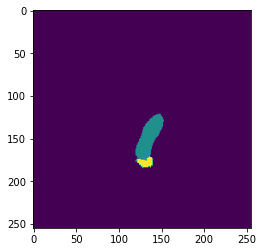
\includegraphics[width = 41mm]{figs/aunet3.png}
    \end{subfigure}
    \begin{subfigure}{.24\linewidth}
    \centering
        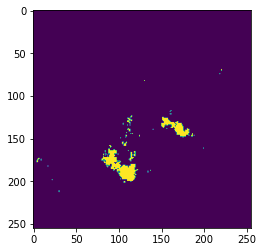
\includegraphics[width = 41mm]{figs/aunet4.png}
    \end{subfigure}
        \begin{subfigure}{.24\linewidth}
    \centering
        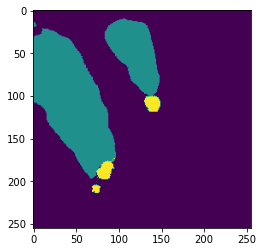
\includegraphics[width = 41mm]{figs/atunet1.png}
    \end{subfigure}
    \begin{subfigure}{.24\linewidth}
    \centering
        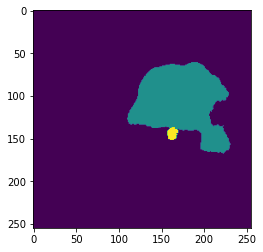
\includegraphics[width = 41mm]{figs/atunet2.png}
    \end{subfigure}
        \begin{subfigure}{.24\linewidth}
    \centering
        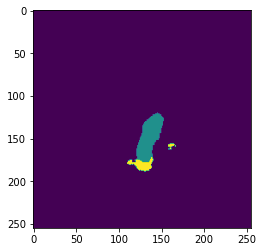
\includegraphics[width = 41mm]{figs/atunet3.png}
    \end{subfigure}
    \begin{subfigure}{.24\linewidth}
    \centering
        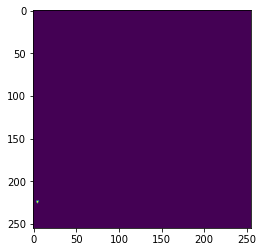
\includegraphics[width = 41mm]{figs/atunet4.png}
    \end{subfigure}
\caption{Segmentation results of ResNet34-based U-net on ground work station. Left two columns: Targets on Kaggle and segmentation results. Right two columns: Experience video data captured by DJI Phantom 4 UAV. Top row: Targets. Mid row: Segmentation results of the designed model. Bottom row: Segmentation results of the designed model developed by attention gates.}
\label{fig:segmentationGround}
\end{figure}\par
As shown in Fig.~\ref{fig:segmentationUAV} is the experience results of the on-board detection. The designed ResNet18 is successfully deployed on DJI M300 UAV. The experience demonstrated that the work of model size decreasing is acceptable. However, the model has not been developed yet. In the first time experience, accuracy is sacrificed to ensure the stable flight and decrease the detection as building the light model. At the start period of experience, the cloud is detected as smoke, which means the model still need more adjustment.
\begin{figure}[ht]
\centering
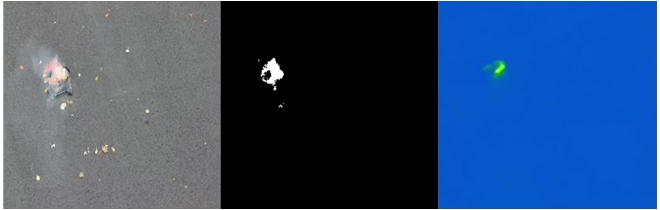
\includegraphics[height=40mm]{figs/test.jpg}
\caption{On-board segmentation result. Left: Masked original image. Mid: Segmentation mask. Right: infrared camera image.}
\label{fig:segmentationUAV}
\end{figure}\par
\subsection{Wildfire Prediction}
The wildfire prediction is based on Cellular model and developed through LSTM. The results could be illustrated in Fig.~\ref{fig:prediction}, it could be demonstrated that the wind impacts the wildfire spreading most heavily.




\end{document}
